% Draft 2 — Boundary-Case Mismatch
% Standalone LaTeX outline for an IJHCS submission.
% Compiles with: pdflatex outline && bibtex outline && pdflatex outline && pdflatex outline
% References file: ../Draft1_NecessityGap/references.bib
\documentclass[11pt,a4paper]{article}
\usepackage[T1]{fontenc}
\usepackage[utf8]{inputenc}
\usepackage{lmodern}
\usepackage[a4paper,margin=2.4cm]{geometry}
\usepackage{microtype}
\usepackage{amsmath,booktabs,array,xcolor,graphicx}
\usepackage{natbib}\bibliographystyle{plainnat}
\usepackage{hyperref}
\hypersetup{colorlinks=true,linkcolor=blue!55!black,citecolor=teal!60!black,
            urlcolor=blue!55!black}
\usepackage{tikz}
\usepackage{pgfplots}\pgfplotsset{compat=1.18}
\usetikzlibrary{arrows.meta,positioning,shadows.blur,calc}

% Palette
\definecolor{bmGreen}{RGB}{56,142,60}
\definecolor{bmAmber}{RGB}{245,124,0}
\definecolor{bmRed}{RGB}{198,40,40}
\definecolor{bmInk}{RGB}{55,65,81}

\title{\textbf{Where the Policy Ends and the User Begins:\\
A Boundary-Case Mismatch in App-Store Privacy Labels}\\[3pt]
\large \textit{Submitted to International Journal of Human-Computer Studies}}
\author{Anonymous Author(s)\\\small Anonymised for review}\date{}
\begin{document}\maketitle

\begin{abstract}\noindent
App-store privacy labels report whether each data category is \emph{collected}
or \emph{shared}. Those binary flags are produced by a chain of
\emph{policy boundary cases} that decide what counts as collection or sharing
in the first place. Using a 87-participant survey on Google Play's nine
boundary cases, we show that the platform and its users disagree about almost
half. Only 48.3\% of users accept off-device ephemeral processing as
non-collection; only 51.7\% accept service-provider transfer as non-sharing;
21.8\% are unsure about anonymised transfer; 14.9\% are unsure even about
prominent-consent-based transfer. Yet Google Play's UI presents the result of
these boundary tests as a binary fact. We name this the \emph{boundary-case
mismatch}: the disclosure can be ``accurate'' in policy terms while remaining
``wrong'' in user terms. We argue that label correctness must be measured at
two layers, policy alignment and user alignment, and we present five
plain-language boundary-explainer patterns derived from the cases where the
mismatch is widest.
\end{abstract}

\noindent\textbf{Keywords:} privacy labels; Data Safety; Google Play;
boundary cases; legal-technical alignment; usable privacy; HCI.

\section{Introduction}
Privacy labels are an \emph{output}. The flag ``shares Location with third
parties'' is the result of a hidden chain of policy decisions: is the recipient
a service provider? Is the transfer user-initiated? Is the data anonymised?
Has consent been collected ``in a way that meets the requirements of Google
Play's User Data policy''? Each link in the chain is a boundary case. Each
boundary case has a policy answer. Each policy answer has a separate user
answer. This paper measures the size of the disagreement.

\section{Boundary Cases Studied}
We test the nine boundary cases that Google Play uses to decide whether a
practice is reported as collection or sharing
(Table~\ref{tab:boundary-cases}).

\begin{table}[h]
\centering\small
\caption{Boundary cases included in the survey.}
\label{tab:boundary-cases}
\begin{tabular}{p{0.30\linewidth}p{0.60\linewidth}}
\toprule
\textbf{Case} & \textbf{Platform-policy claim} \\
\midrule
On-device only & Data is accessed only on the device and is not sent off. \\
End-to-end encryption & Data is sent using E2E encryption. \\
Off-device ephemeral & Data leaves the device but is processed ephemerally. \\
Redirect to service & The app redirects the user to a different service. \\
User-initiated transfer & Transfer is triggered by a user action where transfer
is reasonably expected. \\
Prominent consent & Transfer is disclosed prominently and consent is collected
to platform standards. \\
Service provider & Transfer to a service provider acting on developer's behalf. \\
Legal transfer & Transfer for specified legal purposes. \\
Anonymised transfer & Transfer of fully anonymised data not linkable to an
individual. \\
\bottomrule
\end{tabular}
\end{table}

\section{Method}
Eighty-seven Android users completed a Yes/No/Maybe survey for each of the
nine policy claims, with a short free-text rationale. Yes was operationalised
as agreement with the platform-policy interpretation; Maybe as uncertainty.
Robustness checks remove survey straight-liners ($n=6$ Yes-only, $n=14$
Yes for $\geq25/30$ items) and highly repetitive rationales ($n=25$). All
percentages are computed from the raw \texttt{survey-stats.csv}.

\section{Results}

\begin{figure}[h]
\centering
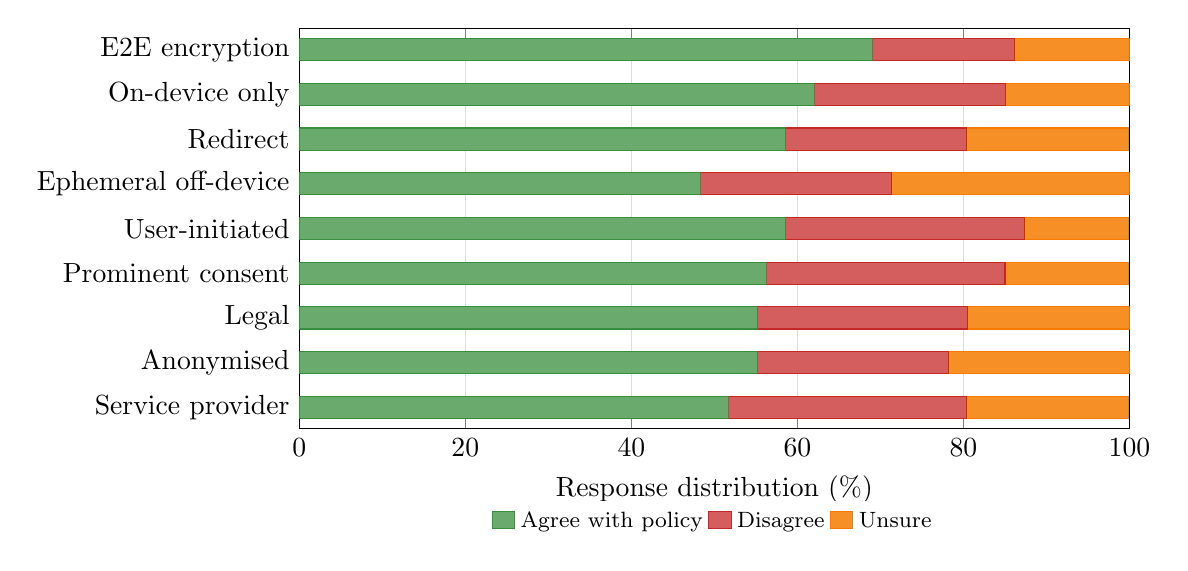
\begin{tikzpicture}
\begin{axis}[
    xbar stacked, width=\linewidth, height=0.55\linewidth,
    xmin=0,xmax=100,xlabel={Response distribution (\%)},
    symbolic y coords={
        Service provider,Anonymised,Legal,Prominent consent,User-initiated,
        Ephemeral off-device,Redirect,On-device only,E2E encryption},
    ytick=data,xtick={0,20,40,60,80,100},
    legend style={at={(0.5,-0.18)},anchor=north,legend columns=3,draw=none,
                  font=\footnotesize},
    bar width=8pt,enlarge y limits=0.06,
    grid=major,grid style={bmInk!18}]
\addplot+[fill=bmGreen!75,draw=bmGreen] coordinates{
  (51.7,Service provider)(55.2,Anonymised)(55.2,Legal)(56.3,Prominent consent)
  (58.6,User-initiated)(48.3,Ephemeral off-device)(58.6,Redirect)
  (62.1,On-device only)(69.0,E2E encryption)};
\addplot+[fill=bmRed!75,draw=bmRed] coordinates{
  (28.7,Service provider)(23.0,Anonymised)(25.3,Legal)(28.7,Prominent consent)
  (28.7,User-initiated)(23.0,Ephemeral off-device)(21.8,Redirect)
  (23.0,On-device only)(17.2,E2E encryption)};
\addplot+[fill=bmAmber!85,draw=bmAmber] coordinates{
  (19.5,Service provider)(21.8,Anonymised)(19.5,Legal)(14.9,Prominent consent)
  (12.6,User-initiated)(28.7,Ephemeral off-device)(19.5,Redirect)
  (14.9,On-device only)(13.8,E2E encryption)};
\legend{Agree with policy, Disagree, Unsure}
\end{axis}\end{tikzpicture}
\caption{Per-boundary-case agreement, disagreement, and uncertainty across the
nine Google Play boundary cases. Where the green portion is below 60\%, the
platform and a substantial share of users disagree about what the label means.}
\label{fig:boundary-cases}
\end{figure}

The clearest cases are end-to-end encryption (69.0\% agree) and on-device-only
(62.1\%). The least clear are off-device ephemeral processing (48.3\% agree,
28.7\% unsure) and service-provider transfer (51.7\% agree, 19.5\% unsure).
Anonymised transfer attracts the highest uncertainty rate (21.8\% Maybe), which
matters because anonymisation is the principal mechanism through which sharing
is legally redefined as non-sharing.

\section{The Boundary-Case Mismatch}
A label is ``accurate'' if the declared facts match the practice as defined by
policy. But for the user it is also a communicative act, and accuracy in that
sense requires that the user reach the same conclusion the policy reaches. We
distinguish two layers (Figure~\ref{fig:mismatch}):

\begin{figure}[h]\centering
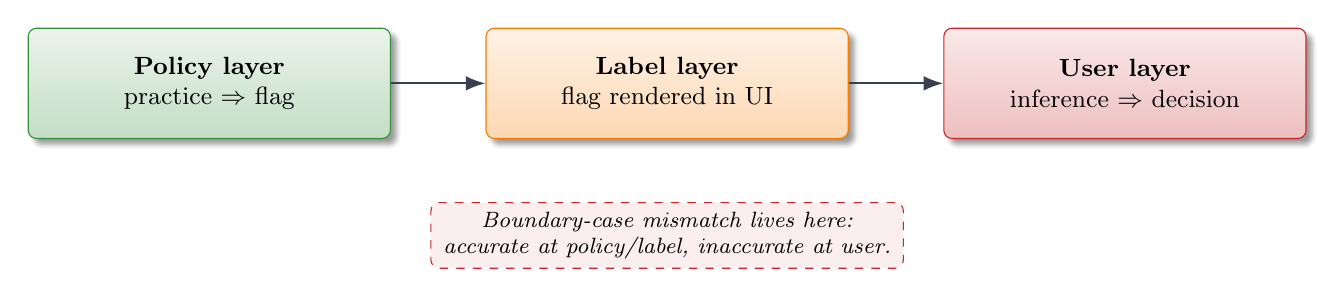
\begin{tikzpicture}[font=\sffamily,
  node distance=10mm,
  L/.style={draw=bmInk,rounded corners=3pt,minimum width=46mm,minimum height=14mm,
            align=center,font=\small,blur shadow={shadow blur steps=4}},
  arr/.style={-{Latex[length=2.5mm]},line width=0.8pt,draw=bmInk}]
\node[L,top color=bmGreen!10,bottom color=bmGreen!30,draw=bmGreen]
  (policy) {\textbf{Policy layer}\\ practice $\Rightarrow$ flag};
\node[L,top color=bmAmber!10,bottom color=bmAmber!30,draw=bmAmber,
      right=12mm of policy]
  (label) {\textbf{Label layer}\\ flag rendered in UI};
\node[L,top color=bmRed!10,bottom color=bmRed!30,draw=bmRed,
      right=12mm of label]
  (user) {\textbf{User layer}\\ inference $\Rightarrow$ decision};
\draw[arr] (policy)--(label);
\draw[arr] (label)--(user);
\node[below=8mm of label,draw=bmRed,dashed,rounded corners=3pt,
      minimum width=60mm,font=\footnotesize\itshape,align=center,
      fill=bmRed!8]
  {Boundary-case mismatch lives here:\\
   accurate at policy/label, inaccurate at user.};
\end{tikzpicture}
\caption{The two-layer accuracy framework. Policy/label accuracy concerns
whether the declared flag is correct under policy. User accuracy concerns
whether the user reaches the same conclusion.}
\label{fig:mismatch}\end{figure}

\section{Design Pattern: Plain-Language Boundary Explainers}
For each of the nine boundary cases, we propose a one-sentence explainer in
\emph{consequence-first} language that drops policy terms in favour of user
consequences: \emph{Does the data leave the device? Who else can access it?
Is it retained? Can it be linked back to me?}

\section{Discussion and Limitations}
This paper does not evaluate a redesigned label; it documents the gap that any
redesign must close. The sample is modest ($N=87$) and recruited from a
crowd-work platform, but the boundary-case findings are stable under quality filters
and offer a
defensible HCI rationale for treating boundary cases as a usability problem,
not a legal formality.

\bibliography{../Draft1_NecessityGap/references}
\end{document}
